\chapter{Bringing pieces together: IL-10-GAG interaction insights}

In this chapter, I assemble important insights about the IL-10-GAG system
derived during this thesis project. Some of these insights have a synergy
effect, i.e.\ they support each other and provide rather strong clues about how
the IL-10-GAG system behaves in nature on the molecular level.


\subsubsection{Experimental input: non-random, but weak interaction}

As noted in \cref{chapter:nmr}, our collaborators in Prof. Huster's NMR
laboratory at the University Leipzig could confirm binding between heparin
oligosaccharides and murine IL-10. As of the high similarity between human and
murine IL-10 (see \cref{background:il10biologyprimer}), this result is very
likely transferable between species. As published \cite{kuenze_gehrcke_2014},
the binding affinity measured in G. Künze's NMR essays was determined to be in
the micromolar range, whereas Salek-Ardakini et al.\ found a binding affinity in
the nanomolar range \cite{salek_ardakani_2000}. Considering the differences in
the investigated systems (polymeric HP \textit{versus} oligomeric HP, human
IL-10 \textit{versus} murine IL-10) and the entirely different experimental
techniques, it is no contradiction that both results differ by an order of
magnitude.

The experimentally obtained binding affinity results and the computationally
obtained observation that IL-10-HP interaction has a measurable impact on the
backbone structure of HP (see \cref{chapter:nmr}) are strong clues that IL-10
and heparin interact in a non-random fashion. However, various indicators point
towards a rather weak interaction when compared to e.g.\ FGF2-HP. One of these
pointers is that HP dp4's iduronic acid populates both, the ${}^1$C${}_4$ and
${}^2$S${}_\mathrm{O}$ conformations in the bound state (see
\cref{chapter:nmr}).


\subsubsection{Putative binding poses are supported by experimental data}

In \cref{chapter:bspred}, a putative IL-10-GAG binding region (occurring twice
as of the symmetry of the IL-10 homodimer) has been proposed, based on the
analysis of IL-10's Coulomb potential. In \cref{chapter:dmd}, it is described
how this binding region was further analyzed with DMD, and narrowed down towards
single key amino acids (being most responsible for GAG binding) and towards two
principal putative GAG binding poses, named A and B (see
\cref{fig:dmdil10:2nd_stage_principal_poses}). These poses are in the
neighborhood of R107, which has been identified as especially important for GAG
binding, and have special relations to experimentally obtained data, as will be
described in the following paragraphs.

\begin{figure}
\centering
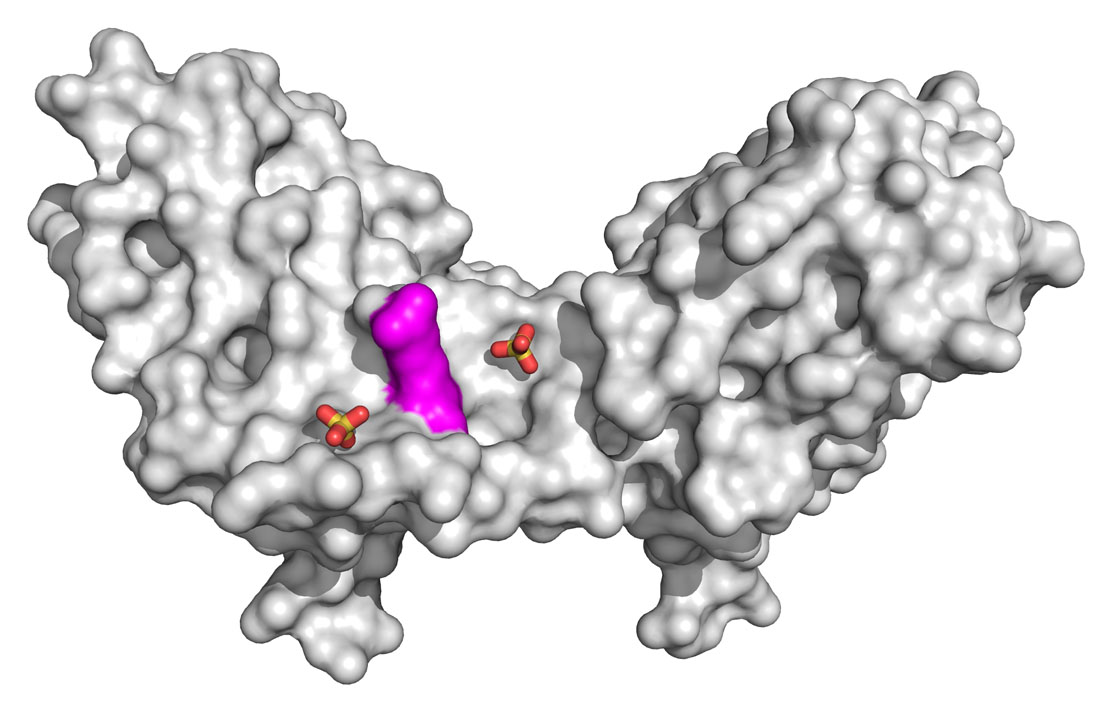
\includegraphics[width=1.0\textwidth]{gfx/together/il10sulfates_01.jpg}
\caption[]{
Structure of human IL-10 according to PDB entry 2ILK in surface representation,
including two sulfate groups contained in the crystal structure, shown in thick
stick representation. The surface of IL-10's amino acid residue R107 is colored
in magenta. }
\label{fig:together:il10sulfates}
\end{figure}

In protein crystallization, salts are often used for diminishing the
electrostatic repulsion and for promoting the hydrophobic interactions among
proteins \cite{crystal_salts_2001}. In high-quality crystal structures, the
atomic groups of salts are spatially resolved and visible. Three sulfate groups
are contained in the 2ILK crystal structure of IL-10 (which has been used
throughout this thesis. Two of these sulfate groups are located right in the
neighborhood of R107, as shown in \cref{fig:together:il10sulfates}.



be concluded that both results fit.


 (two entirely different methods were used) (e.g.\ and )



NMR: IL-10-HP binding happens, measured with lower affinity than initially published by


in orientation A or B, it is more likely that a GAG can bridge both binding
regions.


\subsubsection{Modulation of IL-10 biology by impaired diffusion}
Show image that schematically shows how IL-10 might be caugt by cell-surface-attached GAGs.


\subsubsection{Modulation of IL-10 biology by interference with receptor
binding}

    - Binding region/site
    - Binding features
    - Variation of behavior among GAG types
    - Implications on biology: interference with R2, agglomeration of IL-10
    - Other hypotheses
        - Binding overlaps with R1


\hl{Note (TODO):}
Show picture of R107 specifically marked in the structure, together with
crystal sulfates, discuss possible binding poses involving these crystal
sulfates. Nee, mach das später, bei bringing it all together.

The two binding poses shown in the DMD-IL-10 chapter yeah!


\hl{Note (TODO):}
Discuss models explaining impact of IL-10-GAG interaction on IL-10 biology.



